\documentclass[12pt,fullpage,letterpaper]{article}

\newenvironment{proof}{\noindent{\bf Proof:}}{\qed\bigskip}

\newtheorem{theorem}{Theorem}
\newtheorem{corollary}{Corollary}
\newtheorem{lemma}{Lemma} 
\newtheorem{claim}{Claim}
\newtheorem{fact}{Fact}
\newtheorem{definition}{Definition}
\newtheorem{assumption}{Assumption}
\newtheorem{observation}{Observation}
\newtheorem{example}{Example}
\newcommand{\qed}{\rule{7pt}{7pt}}

\newcommand{\assignment}[4]{
\thispagestyle{plain} 
\newpage
\setcounter{page}{1}
\noindent
\begin{center}
\framebox{ \vbox{ \hbox to 6.28in
{\bf CS446: Machine Learning \hfill #1}
\vspace{4mm}
\hbox to 6.28in
{\hspace{2.5in}\large\mbox{Problem Set #2}}
\vspace{4mm}
\hbox to 6.28in
{{\it Handed Out: #3 \hfill Due: #4}}
}}
\end{center}
}


\newcommand{\handout}[3]{
\thispagestyle{plain} 
\newpage
\setcounter{page}{1}
\noindent
\begin{center}
\framebox{ \vbox{ \hbox to 6.28in
{\bf CS446: Machine Learning \hfill #1}
\vspace{4mm}
\hbox to 6.28in
{\hspace{2.5in}\large\mbox{#2}}
\vspace{4mm}
\hbox to 6.28in
{{\it Handed Out: #3 \hfill Name (NetID): \rule[-2pt]{4cm}{0.1pt} }}
}}
\end{center}
}


\newcommand{\assgsoln}[4]{
\thispagestyle{plain} 
\newpage
\setcounter{page}{1}
\noindent
\begin{center}
\framebox{ \vbox{ \hbox to 6.28in
{\bf CS446: Machine Learning \hfill #1}
\vspace{4mm}
\hbox to 6.28in
{\hspace{2.5in}\large\mbox{Problem Set #2 Solutions}}
\vspace{4mm}
\hbox to 6.28in
{{\it Handed Out: #3 \hfill Handed In: #4}}
}}
\end{center}
}


\newcommand{\solution}[4]{
\thispagestyle{plain} 
\newpage
\setcounter{page}{1}
\noindent
\begin{center}
\framebox{ \vbox{ \hbox to 6.28in
{\bf CS446: Machine Learning \hfill #4}
\vspace{4mm}
\hbox to 6.28in
{\hspace{2.5in}\large\mbox{Problem Set #3}}
\vspace{4mm}
\hbox to 6.28in
{#1 \hfill {\it Handed In: #2}}
}}
\end{center}
\markright{#1}
}


\newenvironment{algorithm}
{\begin{center}
\begin{tabular}{|l|}
\hline
\begin{minipage}{1in}
\begin{tabbing}
\quad\=\qquad\=\qquad\=\qquad\=\qquad\=\qquad\=\qquad\=\kill}
{\end{tabbing}
\end{minipage} \\
\hline
\end{tabular}
\end{center}}

\def\Comment#1{\textsf{\textsl{$\langle\!\langle$#1\/$\rangle\!\rangle$}}}


\usepackage{graphicx}
\graphicspath{{pic/}}
\oddsidemargin 0in
\evensidemargin 0in
\textwidth 6.5in
\topmargin -0.5in
\textheight 9.0in

\begin{document}

\solution{Kaizhao Liang}{\today}{1}{Spring 2017}
% Fill in the above, for example, as follows:
% \solution{Joe Smith}{\today}{1}{Fall 2012}

\pagestyle{myheadings}  % Leave this command alone

\begin{enumerate}
	\item[1.]Learning Conjunctions
	\begin{enumerate}
		\item[a.] My algorithm uses the property of the conjunction, updating the weights by elimination with the positive samples and then verifies them with the negative examples. First of all, my algorithm augments the feature space into 2n, adding the negations of the original features, which makes updating weights more convenient. By the property of conjunction, positive samples could not tolerate any negative feature. In order to maintain the correctness of the prediction, it needs to eliminate the features that are of value 0, i.e. , setting the corresponding weights to 0. In addition, the predictions produced by the remaining features have to be consistent with every label in the negative set. Otherwise, there is not a single conjunction that can satisfiy this data set.\\
		\textbf {Possible Pseudocode:}\\
		Augment the feature space to 2n, where the last n features represent the first n features' negation.\\
		Initialize a weight vector w of length 2n with all 1's.\\
		Separate the data set into two sets with one of only positive samples \(S_+\) and other of only negative samples \(S_-\).\\
		FOR EACH sample \(s\) in \(S_+\):\\
	    \hspace*{5 mm} FOR EACH feature f in s:\\
	    \hspace*{10 mm} IF f==0 THEN\\
	    \hspace*{15 mm} w[f.index]=0\\
	    \hspace*{10 mm}	ENDIF\\
	    \hspace*{5 mm} ENDFOR\\
	    ENDFOR\\
	    \(\theta=\) number of the nonzero elements in w\\
	    FOR EACH sample s in \(S_-\)\\
	    \hspace*{5 mm} prediction= sign of \(w^Ts - \theta\)\\
	    \hspace*{5 mm} IF prediction!=s.label THEN\\
	    \hspace*{10 mm} PRINT OUT "inconsistency message"\\
	    \hspace*{10 mm} BREAK\\
	    \hspace*{5 mm} ENDIF\\
	    ENDFOR\\
		\item[b.] This algorithm either succeeds to find a conjunction or stops when there is no conjunction to satisfy the data set. If it outputs a conjunction, it must be correct, because the elimination, the first loop, guarantees that it will predict all the negative samples right and the verification, the second loop guarantees that it will predict all the positive samples right. If it fails to output a conjunction, it means that there does not exist any conjunction that is consistent with the dataset. Since it's not possible to modify the weights in the verfication without violating the previous samples in the positive set, if the prediction violates the label in the positive set, it coud be concluded that it's not possible to generate a conjunction that fits all the data. Thereby, the correctness of the algorithm is proven.
		\item[c.]Here m is the number of samples and n is the number of features in each sample. Augmenting the feature space takes O(mn). Separating the dataset into two sets takes O(m). Elimination loop takes O(mn). Finding the threshod \(\theta\) takes O(n). Verfication loop also takes O(mn), assuming that the matrix multiplication takes O(n). They added up to O(mn+n). In conclusion, the Running time is O(mn), which is polynomial.
		\item[d.] There might be multiple conjunctions that are consistent with the training data. Since this is an elimination algorithm, it always find the most complicated one, which might include irrelevant features that might lead to an inaccurate prediction for the new data. However, the algorithm should be able to converge, given enough positive samples. As the positive training data grows, the confidence for the hypothesis for the unseen data also grows, when more features are eliminated and the hypothese gets closer to the targeted conjunction.\\
	\item[2.]Linear Algebra Review
	\end{enumerate}
	\begin{enumerate}
		\item[a.]\textbf Suppose there is a point \(x_0\) on the hyperplane such that the \(\|x_0-x_1\|^2\) is minimized, which means either \(x_0=x_1\) or that the vector \((x_0-x_1)\) is perpendicular to the hyperplane:
		\[x_0-x_1=\lambda w\]
		\[\|x_0-x_1\|=\lambda \|w\|\]
		where \(\lambda\) is a constant.\\
		Since \(x_1\) is on the hyperplane:
		\[w^Tx_1+\theta=0\]
		and
		\[x_1=x_0-\lambda w\]
		so
		\[w^T(x_0-\lambda w )+\theta=0\]
		\[\|w^Tx_0+\theta\|=\lambda \|w^Tw\|\]
		Combining the above equations we have:
		\[d=\|x_0-x_1\|=\lambda\|w\|=\frac{\|w^Tx_0+\theta\|}{\|w\|}\]
		\item[b.]\textbf First of all, the two hyperplanes are parallel, because of they share the same \(w\) and since they are parallel, distance between any point of one plane and the other plane is also the distance between the two planes.\\
		Picking random point \(x_0\) on plane \(w^Tx+\theta _1=0\), we have:
		\[w^Tx_0+\theta _1=0\]
		i.e.
		\[w^Tx_0=-\theta _1\]
		 Applying the analytical solution to distance between \(x_0\) and plane \(w^Tx+\theta _2=0\):
		\[d=\frac{\|w^Tx_0+\theta _2\|}{\|w\|}\]
		Substituting the \(w^Tx_0\) with \(-\theta _1\):
		\[d=\frac{\|\theta _2-\theta _1\|}{\|w\|}\]
	\end{enumerate}
	\item[3.]Finding a Linear Discriminant Function via Linear Programming 
	\begin{enumerate}
		\item[a.1.]\textbf{Proof}: Suppose that there exists a plane with w and \(\theta\), such that \(\delta\)=0. Consider the positive sample \(x_+\) and the negative sample \(x_-\) that are closest to the plane.\\
		Since \(y_+(w^Tx_++\theta)\geq 1\) and  \(y_-(w^Tx_-+\theta)\geq 1\),
		\[y_+(w^Tx_++\theta)\geq 1\]
		\[y_-(w^Tx_-+\theta)\geq 1\]
		By the definition of the linear separability, \(y_i(w^Tx_i+\theta)\geq  0\)\\
		Both samples satisfy the above inequalities, hereby that if \(\theta=0\), the data set is linearly separable is proven\\
		Suppose that there exists a hyperplane \(w^Tx+\theta=0\) satisfying the condition \(y_i(w^Tx_i+\theta)\geq 1-\delta \):
		 \[y_i(w^Tx_i+\theta)-1\geq-\delta \]\\
		 Then,\\
		 \[\frac{y_i(w^Tx_i+\theta)-1}{c}\geq\frac{-\delta}{c}\]\\
		 where c is a positive constant.\\
		 Since \(w^Tx_i+\theta-1=0\) and \(\frac{w^Tx_i+\theta-1}{c}=0\) are exactly the same plane, and \(-w^Tx_i-\theta-1=0\) and \(\frac{-w^Tx_i-\theta-1}{c}=0\) are also the same plane, two conditions, \(y_i=0\) and \(y_i=1\), are combined to give:
		 \[\frac{y_i(w^Tx_i+\theta)-1}{c}\geq-\delta\]\\
		 Since c could be any positive number and the assumption is that the data is linearly separable, which means the this hyperplane exists:
		 \[-\delta=-\frac{\delta}{c}\]
		 i.e. \(\delta=0\)\\
		 Hereby that the data is linearly separable iff the \(\delta\) could be optimized to zero is proven.\\
		 \\If there exists a hyperplane that satisfies the condition (3) with \(\delta>0\), the linear separability of the data is uncertain.\\
		 If \(\delta\leq 1\) then the data set is definitely linearly separable and the \(\delta\) can be minimized to 0.\\
		 If \(\delta\geq 1\) then whether the data set is linear separable is not clear, since \(\delta\) could be further minimized.\\
		\item[a.2.] The trivial optimal solution is
					\[w=zeros\]
					\[\theta=0\]\\
					The above solution is correct but useless. To prevent the algorithm from getting this result, the formulation adds some constant c in front of \(-\delta\). The \(c-\theta\) is greater than zero and prevents the left side from converging to zero, thus avoiding the trivial solution. While the value of c does not make great differences as long as it's greater than 0, it only influences the margin.
		\item[a.3.] Given  \(y_i(w^Tx_i+\theta)\geq  1-\delta\) and \(\delta=0\) where ( \(x_1=[1,1,...,1]\),\(y_1=1\) ) and ( \(x_2=[-1,-1,...,-1]\),\(y_2=-1\) ),
		\[y_1(w^Tx_1+\theta )\geq1\]
		\[y_2(w^Tx_2+\theta )\geq1\]\\
		i.e.
		\[\sum w_i + \theta \geq 1\]
		\[\sum w_i -\theta \geq 1\]\\
		Combining the above inequality, it gives solutions:\\
		\[\sum w_i\geq 1\] and \[\theta \geq 1-\sum w_i\]

	\end{enumerate}
	\begin{enumerate}
		\item[b.1.] Rewritting the learning problem:\\
					Given  \(y_i(w^Tx_i+\theta)\geq 1-\delta \), it gives
					 \[y_i(w^Tx_i+\theta)+\delta\geq 1\]\\
					Combining above inequality with \(\delta \geq 0\):
					\[A=[[y_ix_i,y_i,1];[0,0,0,...,1]]\]
					\[t=[w;\theta;\delta]\]
					\[b=[1,1,1,...,0]\]
					where b is of dimension (m+1)x1, and [0,0,0,...,1] is of dimension (n+1)x1.\\
					So \(z(t)=c^Tt=\delta\), which is what needs to be minimized.\\\\
					\textbf{Snippet of function findLinearDiscriminant:}\\\\
					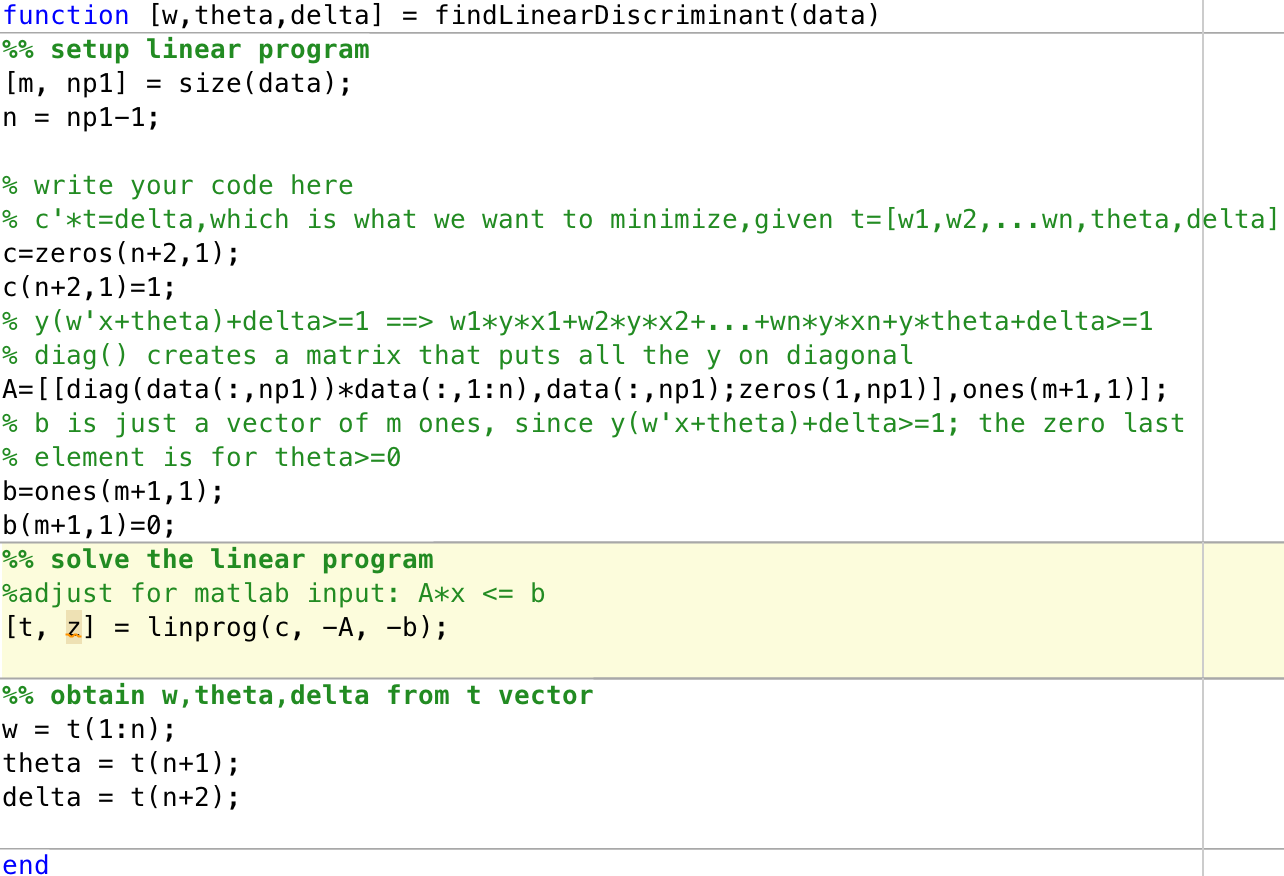
\includegraphics[scale=0.6]{pic/findLinearDiscriminant.png}
		\item[b.2.] \textbf{The data generated:}\\
					1 1 1\\
					1 0 -1\\
					0 1 -1\\
					0 0 -1\\
					\textbf{The figure generated by this data set:}\\
					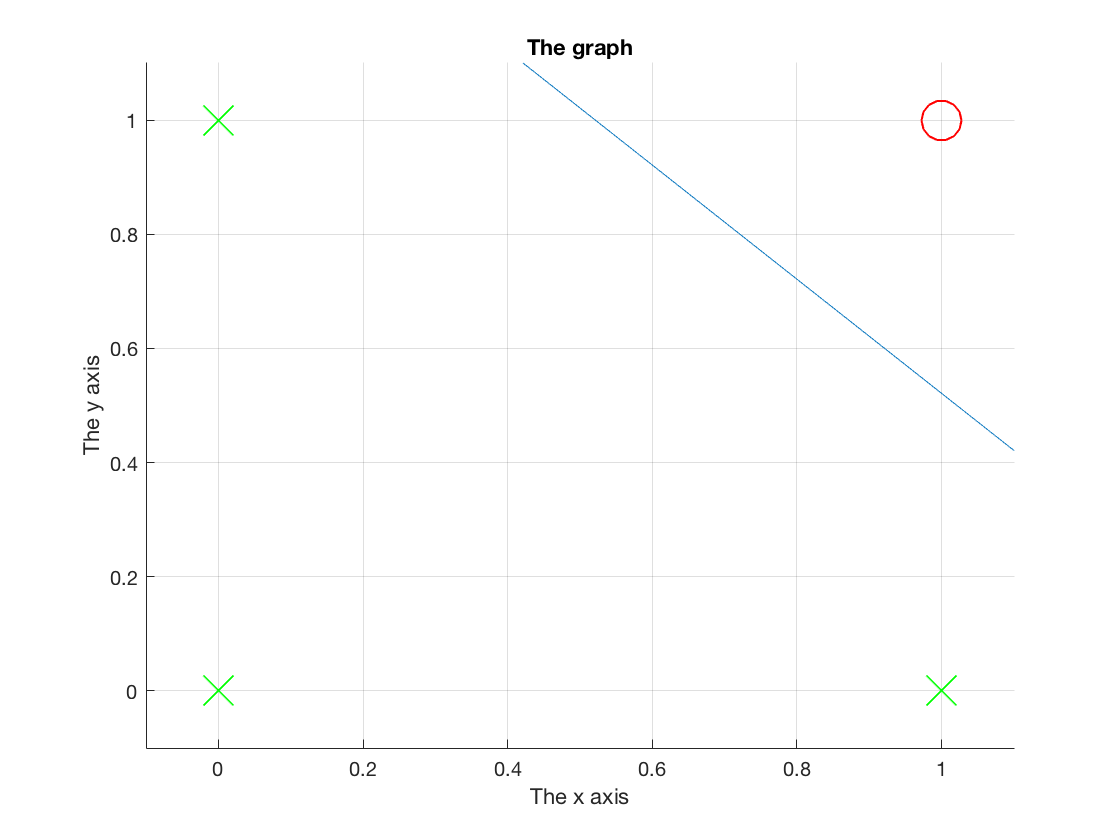
\includegraphics[scale=0.3]{pic/hw1sample2d.png}\\
					\textbf{Snippet of function plot2dSeparator:}\\
					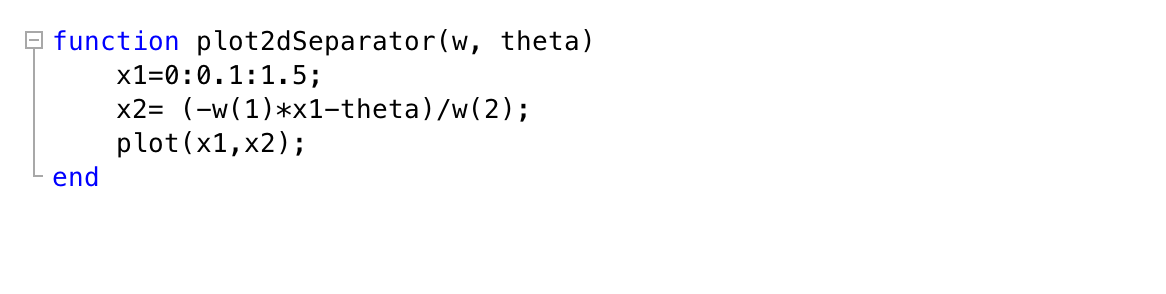
\includegraphics[scale=0.8]{pic/plot2dSeparator.png}\\
					\textbf{Running linear program on hw1conjunction data set outputs:}\\
					\[w=[2.9104,-2.0498,0.1775,190.5196,0.1399,-3.1010,-2.9534,-193.2778,1.1679,-8.8942]\]
					\[\theta=-90.2115\]
					\[\delta=-2.4158\times10^{-13}\]\\
					From the weight above, it's obvious that the conjunction is \(x_4\bigwedge \neg x_8\), since other weights are relatively less significant, while the weights of \(x_4\) and \(x_8\) are exceptionally large, and the sign of the weight determines whether it's negation or not. It's also obivous that \(\delta\approx 0\), indicating that the linear program succeeded in separating the data.
					The threshod \(\theta \approx \frac{\|w_4\|}{2} \approx \frac{\|x_8\|}{2}\) indicates that the program finds the 'best' hyperplane with largest margin possible.\\
		\item[b.3.] \textbf{Snippet of function computeLabels:}\\
					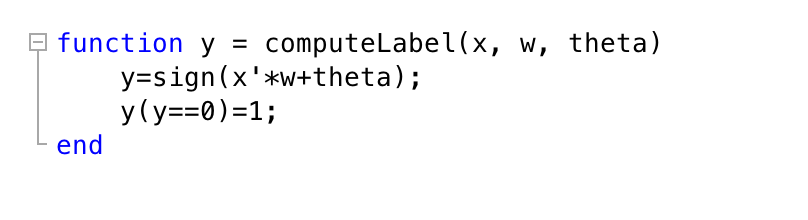
\includegraphics[scale=0.8]{pic/computeLabels.png}\\
					\textbf{The figure generated:}\\
					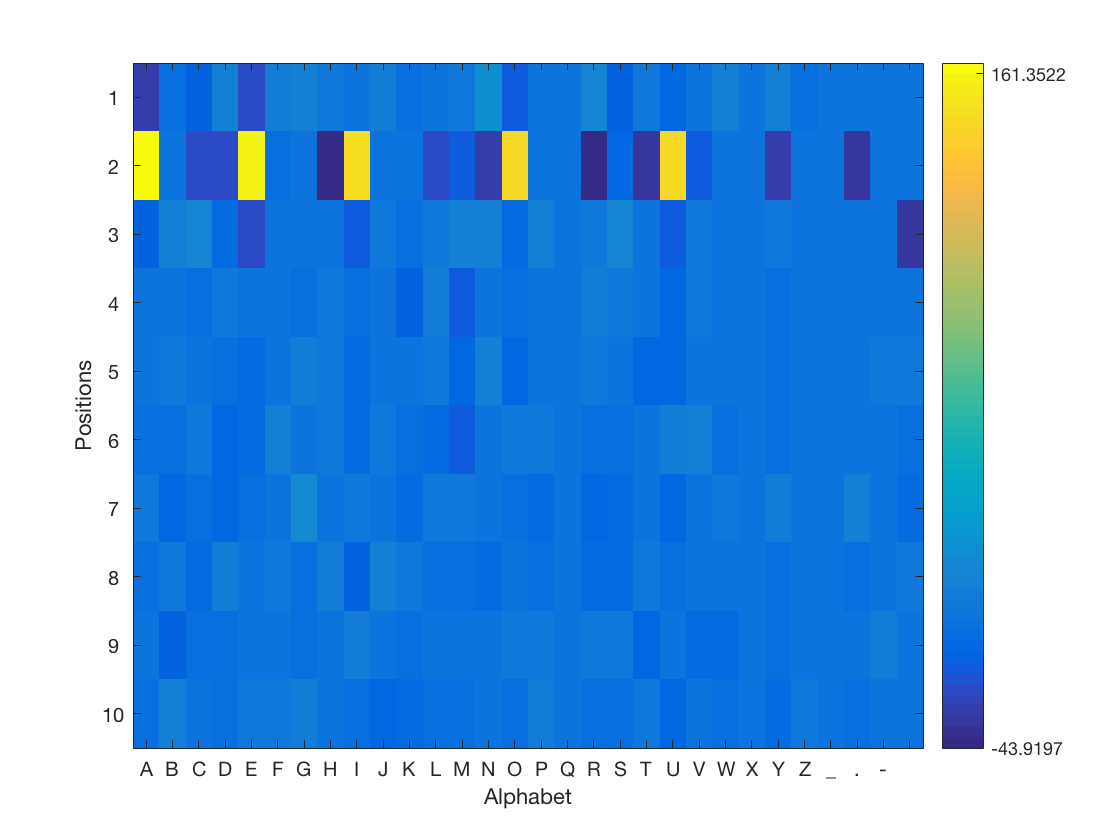
\includegraphics[scale=0.3]{pic/learnBadages.png}\\
					\(\delta=1.2619 \times 10^{-9}\) and \(accuarcyInTrain=1, accuarcyInTest=1\)\\\\
					From the figure above, it is clear that the A, E, I, O, U at position 2 are highlighted, which means that those are the signficant features. \(\delta \approx 0\) indicates the success of the seperation of the data set. The accuarcyInTrain and accuarcyInTest are both 1, i.e. \(100\%\), which implies high confidence in the hypothesis learned.\\\\
					\textbf{After alphabat is changed to BCDEFGHIJKLMNOPQRSTUVWXYZ\_\.\- and position=1:10, figure generated:}\\
					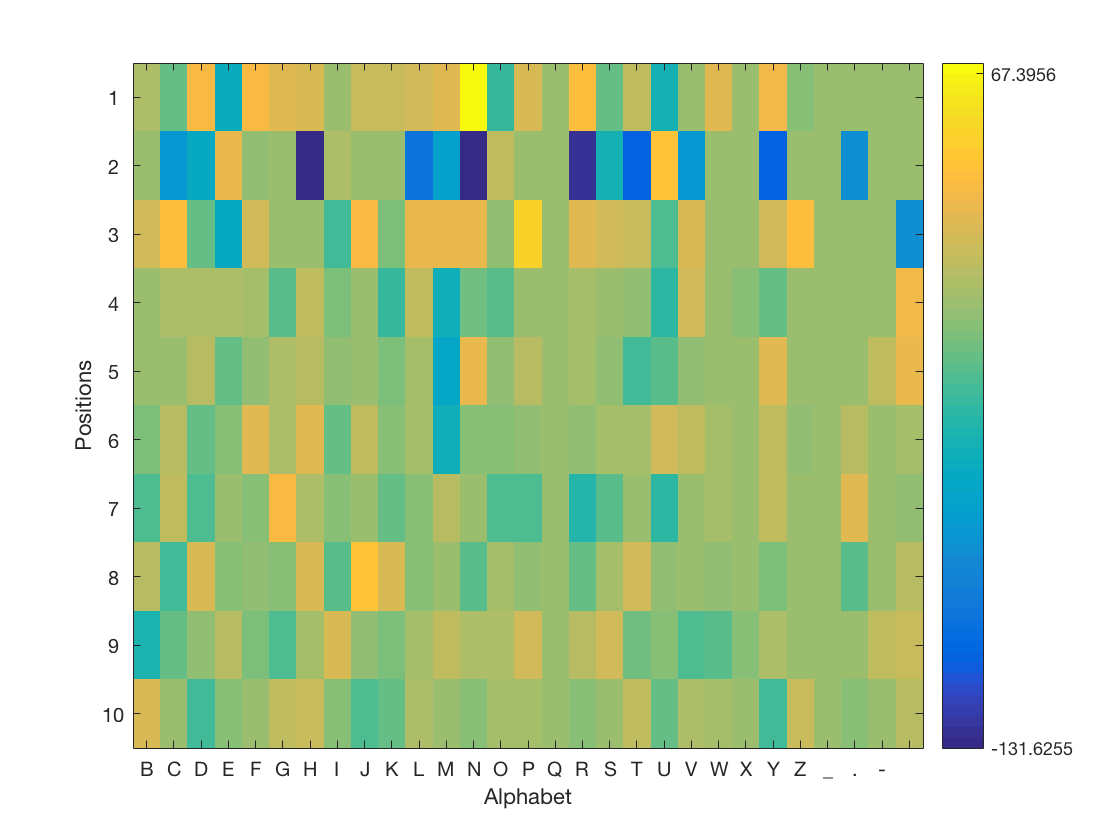
\includegraphics[scale=0.3]{pic/LearnBadages2.png}\\
					\(\delta=4.8317 \times 10^{-12}\) and \(accuarcyInTrain=1, accuarcyInTest= 0.9681\)\\\\
					The figure above is much noiser than the figure obtained before and the weights are more evenly distributed, which means that it's overfitting the training data. However, it still managed to identify two important features, E, U at position 2, and to retreive certain kind of structure that enables it do perform decently in test set.\\
		\item[b.4.]\textbf{Snippet of function findLinearThreshold:}\\
					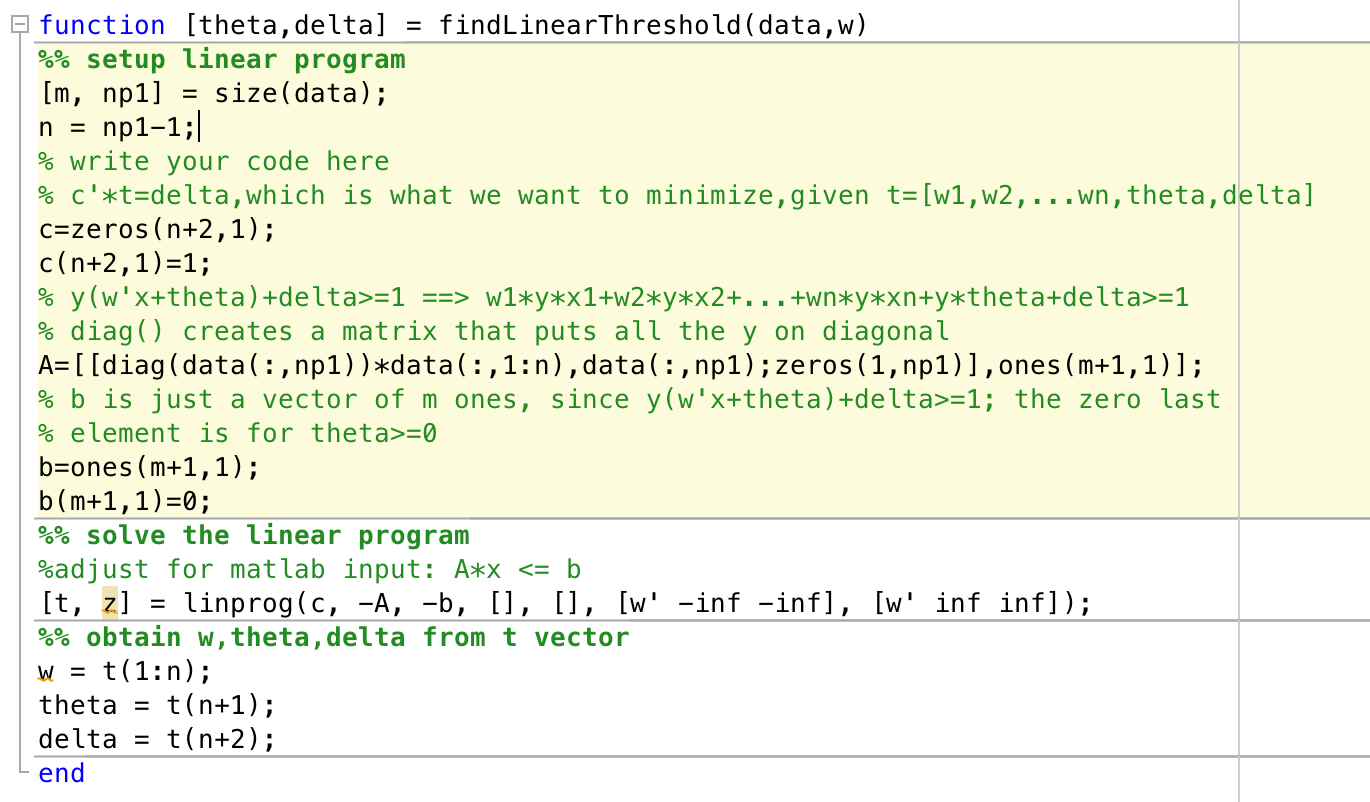
\includegraphics[scale=0.6]{pic/findLinearThreshod.png}\\
					\textbf{The figure generated:}\\
					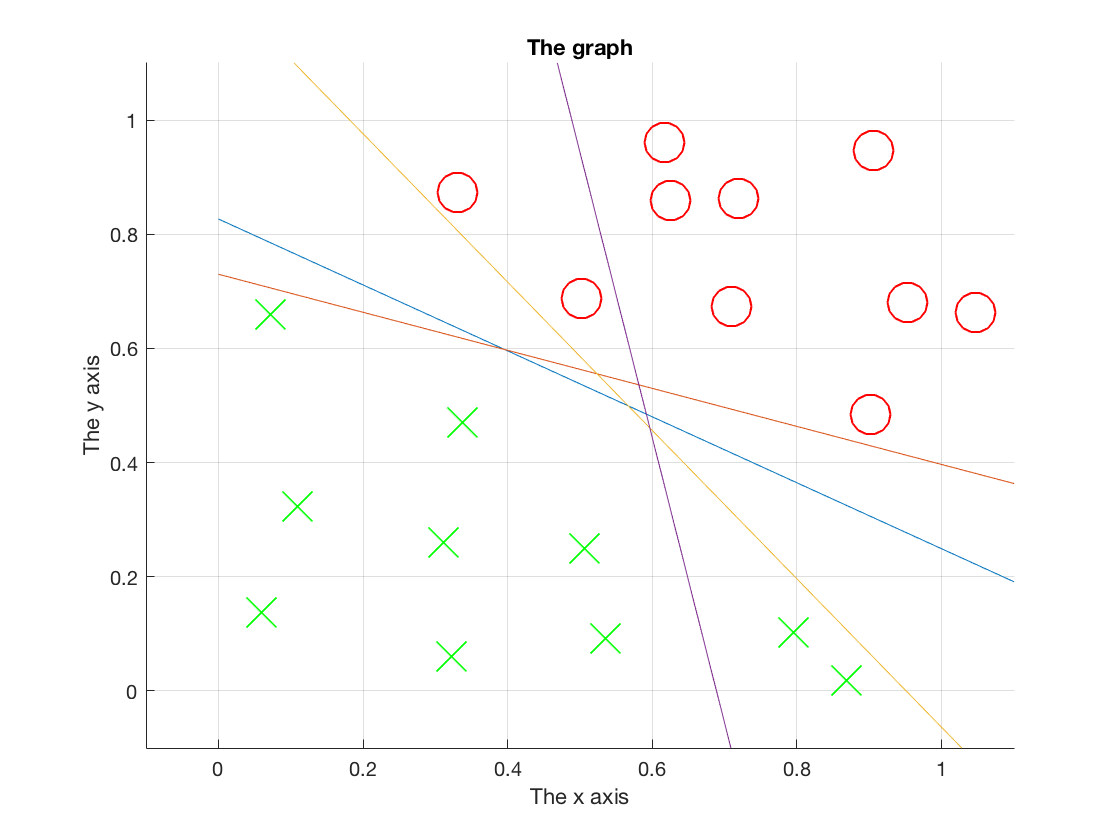
\includegraphics[scale=0.3]{pic/learnMultipleHyperplanes.png}
					\[\delta_1= -1.2506\times 10^{-12},\theta_1= -243.2630\]
					\[\delta_2= -5.1159\times 10^{-13},\theta_2= -218.9946\]
					\[\delta_3= 4.2917\times 10^{-11},\theta_3= -123.6116\]
					\[\delta_4= 92.9650,\theta_4= -344.3350\]\\
					From the above result, it's obvious that except for the purple plane, the other planes successfully separate the data.
					The \(\delta_4\) belongs to the purple hyperplane that fails to separate the data, while the other hyperplanes successfully separate the data and minimize the \(\delta\)s to approximately zero. The \(\delta\) value tells us whether there exist a threshod, such that the hyperplane could separate the data, given a weight. If \(\delta\) could be minimize to 0, there exists a threshod that could enable the hyperplane to separate the data, otherwise, there is no solution.\\\\
					Empirically, the blue hyperplane is the best, since it has the largest margin, which presumably is mroe generalized and is more likely to predict correctly when encountering a new unseen sample, while the others have too strict a condition and very likely to misclassify.\\\\
					From the above examples, it's evident that the solution of the LP is not unique. Given different weights, the \(\delta\) could all be minimizd to approximately 0. So all the weights that satisfy this condition could be solution.
	\end{enumerate}
\end{enumerate}

\end{document}

